\documentclass[letterpaper, 12pt]{article}

\usepackage{geometry}
 \geometry{
 letterpaper,
 total={170mm,257mm},
 left=20mm,
 top=20mm,
 bottom=20mm
 }
\usepackage{graphicx} % Required for inserting images
\usepackage{authblk}
\usepackage{amssymb}
\usepackage{lipsum}
\usepackage{float}
\usepackage{times}
\usepackage{amsmath}
\usepackage[format=plain,
            labelfont={bf,it},
            textfont=it]{caption}
\captionsetup{justification=raggedright,singlelinecheck=false}
\usepackage{ragged2e}
\usepackage{longtable}
\usepackage{comment}
\usepackage{setspace}
\usepackage{fancyhdr}
\usepackage{titlesec}
\usepackage[hyperindex,breaklinks]{hyperref}
\hypersetup{
    colorlinks=true,
    linkcolor=blue,
    filecolor=magenta,      
    urlcolor=blue,
    pdftitle={Overleaf Example},
    pdfpagemode=FullScreen,
    }
% \usepackage{background} % add COSIG logo to page
\usepackage[T1]{fontenc}
\usepackage{helvet}
\renewcommand{\familydefault}{\sfdefault}
\pagenumbering{gobble}
\usepackage[skip=10pt plus1pt, indent=40pt]{parskip}

\titlespacing*{\section}
{0pt}{1.5ex plus 1ex minus .2ex}{1.3ex plus .2ex}

\renewcommand\Authfont{\fontsize{12}{14.4}\selectfont}
\renewcommand\Affilfont{\fontsize{9}{10.8}\itshape}
 
\begin{document}
\flushleft

\includegraphics[width=0.5\textwidth]{img/home/241017_final_logo_mockup.png}

\section*{Tumor burden}
\addcontentsline{toc}{section}{Tumor burden}
\textit{Last updated: 4 April 2025}

\textit{Note: This guide contains images of tumor-bearing laboratory animals and excised tumors that some readers may find disturbing.}

Cancer research often involves implanting, injecting or otherwise inducing tumors in rodent models. To minimize the suffering of the animals involved, \href{https://en.wikipedia.org/wiki/Institutional_Animal_Care_and_Use_Committee}{Institutional Animal Care and Use Committees} (IACUCs), also called Animal Ethics Committees (AECs) and Animal Welfare and Ethical Review Body (AWERBs), establish guidelines on tumor burden that researchers at the institution must follow. Most institutions require protocols to be approved by their IACUC before any animal experiments are performed. These approvals come with a number that is often, but not always, reported in the article reporting on the experiments. Authors and institutions should be able to furnish this number and ethical approval documents if requested.

Guidelines by institution vary in specifics, but generally require that:

\begin{itemize}
    \setlength\itemsep{-0.5em}
    \item \textbf{Tumors should not be implanted in certain areas on an animal.} These areas include the face, the limbs, the ventral surface (where tumors may drag against the enclosure floor and bedding), the genitalia and within muscles (where tumor growth could cause painful muscular distension). Tumor placement should not interfere with normal bodily functions like walking, eating, drinking, urinating and defecating.
    \item \textbf{Tumors should not exceed a maximum size/volume.} Limits on tumor size vary between institutions and for different species. Generally, tumors should not measure more than 2.0 cm across their longest axis for mice and more than 4.0 cm across their longest axis for rats and should not exceed a volume of 2000 mm$^3$ for mice and 4000 mm$^3$ for rats. If multiple tumors are present, the sum of the maximum diameters and volumes of each tumor is usually considered (i.e., a mouse with one tumor with a volume of 1,800 mm$^3$ would fall within ethical guidelines, but two two tumors each with a volume of 1,800 mm$^3$, a combined volume of 3,600 mm$^3$, would not). Alternatively, many institutions suggest that tumors should not grow to be more than 15\% of an animal's body weight. Animals that grow tumors above these thresholds should be euthanized immediately.
    \item \textbf{Animals should not lose excessive weight, showcase behavior indicating distress or display skin lesions.} There are a variety of clinical signs indicating that an animal is suffering or that a tumor has altered an animal's health status. Many of these are described in \href{https://animalcare.jhu.edu/wp-content/uploads/sites/5/Tumor-Study-Guidelines-in-Mice-and-Rats.pdf}{Johns Hopkins University's Tumor Study Guidelines}.
    \item \textbf{Animals should be observed and tumors should be measured on a regular basis.} Tumors can grow very quickly. Most institutions require animals to be observed at least twice weekly to monitor tumor progression and animal health.
\end{itemize}

Tumor size limits instituted and recommended by various authorities are summarized in the table below.

\begin{center}
\begin{tabular}{|p{5.2cm}|p{5.2cm}|p{5.2cm}|}
\hline
     Authority & Max diameter (mice/rats) & Max volume (mice/rats) \\ \hline\hline
     \href{https://iacuc.ucsf.edu/sites/g/files/tkssra751/f/wysiwyg/GUIDELINE%20-%20Tumor%20Induction%20in%20mice%20and%20rats.pdf}{University of California San Francisco (2022)} & 2.0 cm / 4.0 cm & - \\ \hline 
     \href{https://animalcare.jhu.edu/wp-content/uploads/sites/5/Tumor-Study-Guidelines-in-Mice-and-Rats.pdf}{Johns Hopkins University (2024)} & 2.0 cm / 4.0 cm & 4000 mm$^3$ / 36,000 mm$^3$ \\ \hline
     \href{https://doi.org/10.1038/sj.bjc.6605642}{UK National Cancer Research Institute (2010)} & 1.5 cm / 2.8 cm* & - \\ \hline
     \href{https://policies.unc.edu/TDClient/2833/Portal/KB/ArticleDet?ID=132214}{University of North Carolina at Chapel Hill (2019)} & 2.0 cm / 4.0 cm & 2000 mm$^3$ / 5000 mm$^3$ \\ \hline
\end{tabular}
\end{center}
\textit{* Measured as the mean of the major axis and minor axis of the tumor.}

When images of excised tumors or subcutaneous tumors are shown in an article alongside scale bars, tumor volume can be estimated by measuring the long axis $D$ and short axis $d$. Volume is commonly approximated by $V = d^2D/2$.

\pagebreak

\subsection*{Example 1: Mouse tumors exceeding humane limits, shown in images}

\href{https://doi.org/10.3389/fonc.2020.00415}{Si et al. (2020)} report on experiments in \href{https://en.wikipedia.org/wiki/C57BL/6}{C57BL/6 mice} in which the mice were injected with a mouse melanoma cell line in their right flank. Several images shown in the article suggest that these tumors were allowed to grow extremely large. The images shown of mice also suggest the tumors likely inhibited the animals' ability to walk. The article claims that ``[the] animal study was reviewed and approved by Shihezi University Animal Care and Use Committee''.

\begin{figure}[h!tbp]
    \centering
    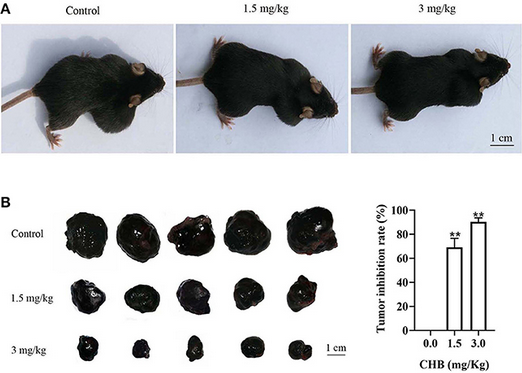
\includegraphics[width=0.8\textwidth]{img/tumor_burden/Screenshot 2025-04-04 at 15-23-31 fonc-10-00415-g006.png}
    \caption*{Images of tumor-bearing mice and excised tumors from \href{https://doi.org/10.3389/fonc.2020.00415}{Si et al. (2020)}. The excised tumors reach up to nearly 3.0 cm across their longest axis. Estimating the longest tumor shown to have a major axis length of 3.0 cm and a minor axis length of 3.0 cm, these tumors likely reached volumes up to 13,500 mm$^3$. Adapted from Figure 6 of Si et al.}
\end{figure}

\pagebreak

\subsection*{Example 2: Mouse tumors exceeding humane limits, shown in images and data}

\href{https://doi.org/10.3390/app13021090}{Su et al. (2023)} report on experiments in \href{https://www.jax.org/strain/007850}{athymic nude mice} where the mice were implanted with a human squamous cell carcinoma cell line in their right hip. A chart shown in Figure 4 of the article suggests that mice were allowed to grow tumors exceeding 6000 mm$^3$ in volume. The article claims ``[these] animal studies were performed with the approval of the Animal Experimentation Ethics Committee of Daegu Haany University (Gyeongsan-si, Republic of Korea) (approval no. DHU2017-098)''.

\begin{figure}[h!tbp]
    \centering
    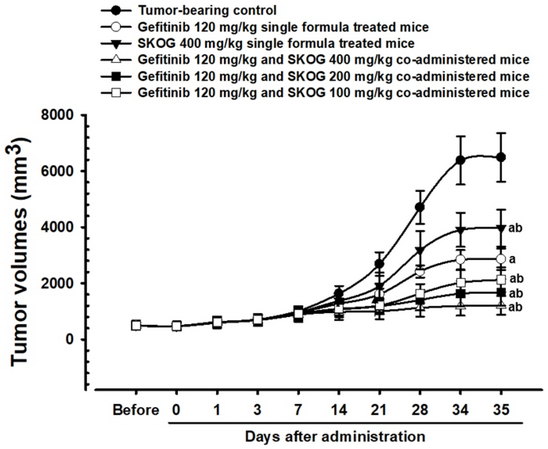
\includegraphics[width=0.8\textwidth]{img/tumor_burden/Screenshot 2025-04-04 at 15-50-26.png}
    \caption*{\href{https://doi.org/10.3390/app13021090}{Su et al. (2023)} show data that suggest that mice were allowed to grow tumors having volumes well in excess of humane limits. Images shown in the article of tumor-bearing animals confirm that these tumors were extremely large. Adapted from Figure 4 of Su et al.}
\end{figure}

\subsection*{Additional resources}

\begin{itemize}
    \setlength\itemsep{-0.5em}
    \item \href{https://scienceintegritydigest.com/2020/05/07/animal-ethics-misconduct-mice-with-very-large-tumors/}{``Animal ethics misconduct: mice with very large tumors'' (2020)}
\end{itemize}

\end{document}